\documentclass[12pt]{article}

\usepackage{graphicx} %Imágenes
\usepackage[utf8]{inputenc} %Tildes
\usepackage[spanish,es-tabla]{babel} %Español, es-table: llamar tablas en vez de cuadros
\usepackage[breaklinks=true]{hyperref} %Hiperenlaces
\usepackage{amssymb, amsmath, amsbsy} %Símbolos matemáticos
\usepackage{float} %Mover las imágenes usando [H]
\usepackage{eurosym} %Símbolo de euro \euro
\usepackage{listings} %Código
\usepackage{listingsutf8} %Tildes en listings
\usepackage{tikz} %Dibujos
\usetikzlibrary{matrix} %Dibujos
\usepackage{algorithm} %Pseudocódigo
\usepackage{algpseudocode} %Pseudocódigo
\usepackage[shortlabels]{enumitem} % Enumerates con a) 	\begin{enumerate}[a)]
\usepackage{multimedia}

\usepackage{amsmath}
\usepackage{graphicx}
\usepackage{hyperref}
\usepackage[utf8]{inputenc}
\usepackage[spanish]{babel}
\usepackage[margin=3cm]{geometry}
\usepackage{amsfonts}
\usepackage{listings}
\usepackage{textcomp}
\usepackage{float}

\title{Ideology Algorithm.}
\author{Míriam Mengíbar Rodríguez - \href{mailto:mirismr@correo.ugr.es}{mirismr@correo.ugr.es}\\Néstor Rodríguez Vico - \href{mailto:nrv23@correo.ugr.es}{nrv23@correo.ugr.es}}
\date{\today}

%\begin{algorithmic} dentro de \begin{codigo} \end{codigo}
\newenvironment{codigo}
 {\par\addvspace{\topsep}
  \centering
  \begin{minipage}{\linewidth}
  \hrule\kern2pt}
 {\par\kern2pt\hrule
  \end{minipage}
  \par\addvspace{\topsep}}

\numberwithin{figure}{section} %Hace que la primera figura de cada sección X sea X.1
\numberwithin{table}{section} %Hace que la primera tabla de cada sección X sea X.1

\begin{document}
	\maketitle
	
	\setlength{\belowdisplayskip}{5pt} 
	\setlength{\belowdisplayshortskip}{5pt}
	\setlength{\abovedisplayskip}{5pt} 
	\setlength{\abovedisplayshortskip}{5pt}

	\section[Introducción al algoritmo.]{Introducción al algoritmo.}
	
	El algoritmo estudiado en este trabajo se llama \textit{Ideology Algorithm}. Fue desarrollado en el año 2016 por los autores Teo Ting Huan, Anand J. Kulkarni, Jeevan Kanesan, Chuah Joon Huang y Ajith Abraham. Se trata de un algoritmo poblacional diseñado para problemas de optimización real. Es un algoritmo basado en el comportamiento de los políticos. La idea es tener una población de individuos (políticos) agrupadas en subpoblaciones (partidos políticos) la cual va evolucionando según la interacción que se produce entre los individuos de la misma. Las distintas subpoblaciones se mantienen ordenadas por como de buenos son los individuos y así podemos identificar cinco tipos de individuos: el líder, el sublíder, el peor, el segundo peor y el resto de individuos. Dentro de la población llamaremos el líder global al mejor individuo de todos. Durante las iteraciones del algoritmo cada individuo genera nuevos individuos de una forma distinta:
	
	\begin{itemize}
	\item El líder, de forma análoga a la vida real, intentará mejorar el sólo (proceso llamado introspección), intentará mejorar fijándose en el sublíder de su partido para intentar seguir siendo el mejor (competición local) y intentará mejorar fijándose líder global para llegar a ser el líder global (competición global).
	\item El peor individuo comprobará si debe seguir en el partido político en el que se encuentra o debe marcharse a otro. Para ello se fijará en cómo de diferente es su forma de pensar (el valor de la solución) con respecto al segundo peor individuo del partido. Si la diferencia es mayor que un umbral, este se marchará a un partido elegido de forma aleatoria.
	\item El resto de individuos intentará mejorar por sí mismos (proceso llamado introspección) e intentarán mejorar fijándose en el líder de su partido (competición local).
	\end{itemize}
	
	Un pequeño pseudocódigo del algoritmo sería el siguiente:
	
	\begin{codigo}
	\begin{algorithmic}[1]
	\Function {IdeologyAlgorithm}{}
	\State Generación de los individuos
	\State Reparto en los partidos
	\While{no hay convergencia}
	\State Evaluamos los individuos
	\State Los ordenamos en función del valor de la solución
	\State Actualización de los líderes
	\State Vemos si algún político tiene que cambiar de partido
	\State Actualización del resto de los individuos
	\EndWhile
	\EndFunction
	\end{algorithmic}
	\end{codigo}

	Como podemos ver el pseudocódigo es bastante simple y sique el esquema de cualquier algoritmo genético, con unas pequeñas adaptaciones concretas de este algoritmo.
	
	\section[Proceso desarrollado.]{Proceso desarrollado.}
	
	Los resultados que se van a mostrar a continuación se han obtenido con una implementación propia del algoritmo en \textit{Python}. Para la evaluación de nuestro algoritmos se usado el módulo \textbf{optproblems}. Se trata de un módulo el cual tiene diferentes funciones usadas en problemas de optimización, entre las cuales se encuentras las usadas en la competición \textit{CEC} del año 2005, que son las funciones usadas por los autores de nuestro paper. \\
	
	En nuestra implementación hay cosas que no han quedado claras del todo en el paper así que hemos tenido que hacer lo que hemos considerado más oportuno. Por ejemplo, el umbral que determina cuando un político cambia de partido no viene dado y el valor de R (un factor usado para la creación de los nuevos individuos) es de 0.000001, lo cual no tiene sentido. Veamos un ejemplo de su uso y comentemos por qué no lo tiene: 
	
	\begin{equation} \label{equation}
		\psi _{i, insp}^{L_{p,b}} \in \left [ x_{i}^{L_{p,b}} - R \left ( \left \| \psi _{i}^{u, p} \right \| - \left \| \psi _{i}^{l, p} \right \| \right ), x_{i}^{L_{p,b}} + R \left ( \left \| \psi _{i}^{u, p} \right \| - \left \| \psi _{i}^{l, p} \right \| \right ) \right ]
	\end{equation}
	
	La idea es generar un intervalo, $\psi _{i, insp}^{L_{p,b}}$, en el cual se va a mover la nueva solución. Como podemos ver, la única diferencia del límite superior e inferior es que se sume o se reste el producto de $R$ por $\left ( \left \| \psi _{i}^{u, p} \right \| - \left \| \psi _{i}^{l, p} \right \| \right )$. Si \textit{R} vale 0.000001, ese producto va a dar un valor cercano a cero y si dicho valor se lo sumamos o restamos a $x_i$ vamos a tener que el límite superior y el inferior son prácticamente idénticos y cuando intentemos generar una solución en ese rango, la solución va a casi coincidir con alguno de los límites del intervalo y, por lo tanto, con el individuo original. Esto produce que el algoritmo se estanque muy rápido, ya que los intervalos se van cerrando con el paso de las iteraciones. Para que esto no suceda, hemos inicializado $R$ a 0.05 (valor obtenido empíricamente tras varias pruebas). \\ 
	
	El umbral de deserción tampoco viene dado. Dicho umbral define cuando un político dal el salto a otro partido. En nuestro caso, lo hemos fijado a 10, ya que tras hacer varios experimentos es el que mejor resultados nos ha dado.
	
	\section[Detalles.]{Detalles.}
	
	En esta sección vamos a comentar los detalles del algoritmo. Veamos las partes clásicas de un algoritmo evolutivo a ver si aplican:
	
	\begin{itemize}
		\item \textbf{Inicialización de la población}: Creamos tantos individuaos (políticos) como indicado en el argumento de entrada. A continuación, aplicamos un algoritmo \textit{k-Means} para crear tantos \textit{clústers} (partidios políticos) como los indicados en el arguemento de entrada. Este algoritmo \textit{k-Means} debe garantizar que los \textit{clústers} tengan los mismos elementos. 
		\item \textbf{Representación de un individuo}: Dado que nos encontramos frente a un problema de optimización real, un individuo está representado mediante un vector de valores reales. Dichos valores son se mueven en un intervalo específicado por la propia función a optimizar en la documentación de la competición \textit{CEC}.
		\item \textbf{Operador de cruce}: En este caso no tenemos un operador de cruce como tal para generar nuevos individuos. Estos individuo se generan modificando los valores de los mismos en base a la equación \ref{equation}.
		\item \textbf{Operador de selección}: En este caso tampoco tenemos un operador de selcción como tal para cruzar individuos, ya que los nuevos individuos no se generan cruzando a varios individuos existentes. El algoritmo modifica todos los individuos, así que no hay un operador de selección definido. Si es cierto que la generación de un nuevo individuo se produce o no en función de la generación de un número aleatorio, así que puede darse el caso de que ciertos individuos o ciertas componentes de los mismos no sean actualizadas.
		\item \textbf{Función de evaluación}: La función de evaluación usada es la función elegida de la competición \textit{CEC}. En nuestra implementación, dicha función es un argumento, permitiendo así que ejecutar el algoritmo con cualquier función.
		\item \textbf{Terminación}: el algoritmo termina cuando se han realizaco \textit{N} llamadas a la función de evaluación.
	\end{itemize}
	
	\section[Resultados.]{Resultados.}
	
	Como se ha comentado anteriormente, para evaluar la eficacia de este algoritmos se han suado las funciones las funciones del \textit{CEC2005}, las cuales podemos ver definidas en su \textit{Tech Report}, el cual podemos encontrar \href{http://www.cmap.polytechnique.fr/~nikolaus.hansen/Tech-Report-May-30-05.pdf}{aquí}. Para no abrumar con los resultados, sólo vamos a mostrar las funciones más relevantes, ya sea por su buen o por su mal resultado. \\
	
	Para los experimentos se han usado \textit{10000*dimensión del problema} evaluaciones, cinco partidos políticos y 150 políticos. A continuación, vamos a mostrar los resultados obtenidos para las funciones más relevantes de nuestro problema:
	
	\begin{table}[H]
		\centering
		\begin{tabular}{rcccc}
			\textbf{} & \multicolumn{2}{c}{\textbf{Dimensión 10}} & \multicolumn{2}{c}{\textbf{Dimensión 10}} \\ \cline{2-5} 
			\textbf{Función} & \textbf{Mínimo} & \textbf{Valor obtenido} & \textbf{Mínimo} & \textbf{Valor obtenido} \\ \hline
			1 & -450.0 & -448.9383774659622 & -450.0 & -440.2389984719936 \\
			2 & -450.0 & -449.1681084750577 & -450.0 & -411.95544114220314 \\
			5 & -310.0 & -278.7341595213256 & -310.0 & 4111.7098960347585 \\
			6 & 390.0 & 397.4416234745711 & 390.0 & 8275.165416601421 \\
			8 & -140.0 & -119.4496863523056 & -140.0 & -118.99854747151608 \\
			9 & -330.0 & -310.5566575168368 & -330.0 & -66.15589012073474 \\
			10 & -330.0 & -318.8687785901725 & -330.0 & -166.33617024989627 \\
			11 & 90.0 & 92.76632067114448 & 90.0 & 106.3562203027524 \\
			13 & -130.0 & -129.01951580640508 & -130.0 & -123.29255503352549 \\
			14 & -300.0 & -296.0181343351546 & -300.0 & -286.02902111474947 \\
			17 & 120.0 & 155.88408833604626 & 120.0 & 186.6069262528208 \\
			22 & 360.0 & 1171.2463561690809 & 360.0 & 1250.035657273889 \\
			24 & 260.0 & 460.0088039230323 & 260.0 & 460.36508779474815
		\end{tabular}
	\end{table}
	
	Como podemos ver, en ciertas funciones alcanzamos el mínimo y en otras nos quedamos cerca. Aún así, el algoritmo no es infalible, por ejemplo, en la función 22 el mínimo está en \textit{360} y el algoritmo obtiene un valor de \textit{1171.246356169081}.\\
	
	Una vez hemos visto los resultados, vamos a ver unas gráficas de convergencia para ver como va evolucionando el valor de la función objetivo del mejor individuo (el líder global). 
	
	\begin{table}[H]
	\centering
	\begin{tabular}{ll}
	\includegraphics[width=0.5\linewidth]{./images/f5_dim10.eps} & 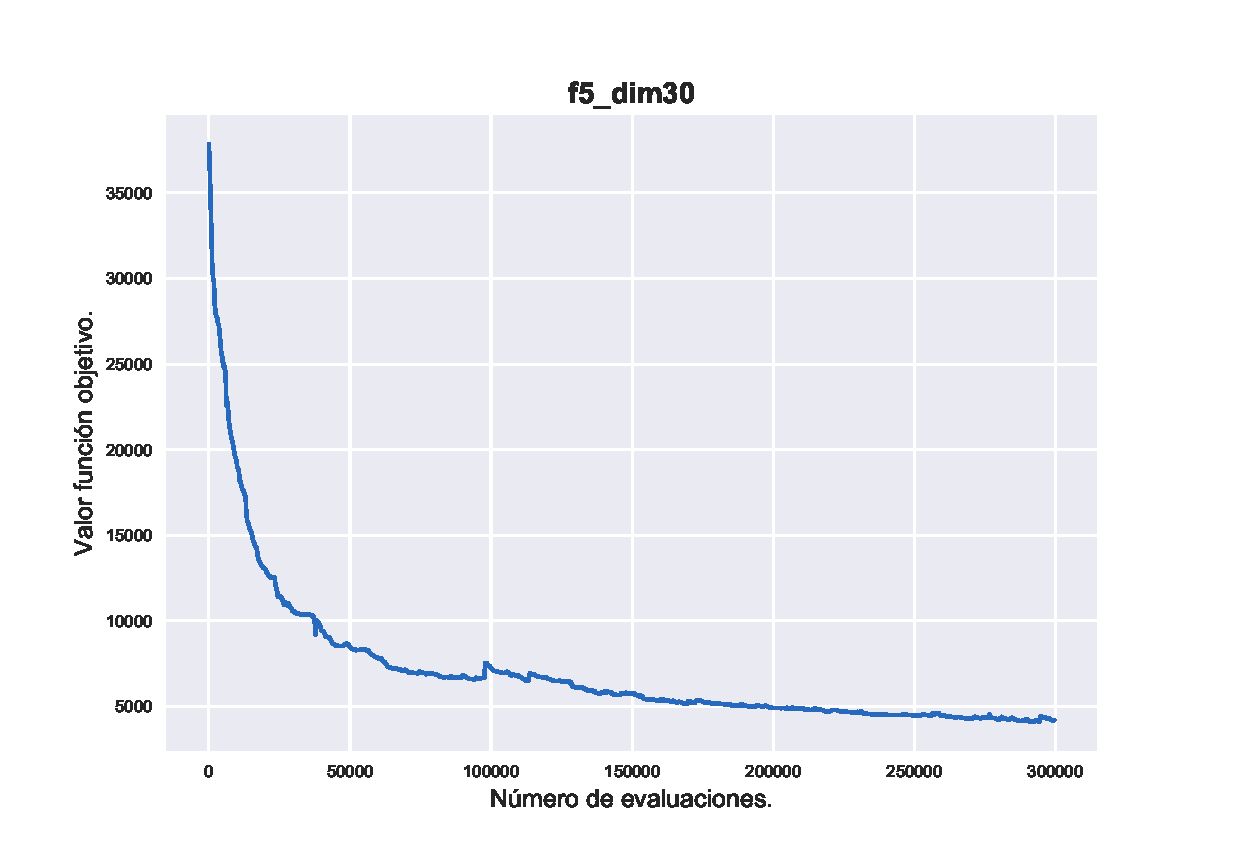
\includegraphics[width=0.5\linewidth]{./images/f5_dim30.eps} \\
	\end{tabular}
	\end{table}

	\begin{table}[H]
	\centering
	\begin{tabular}{ll}
	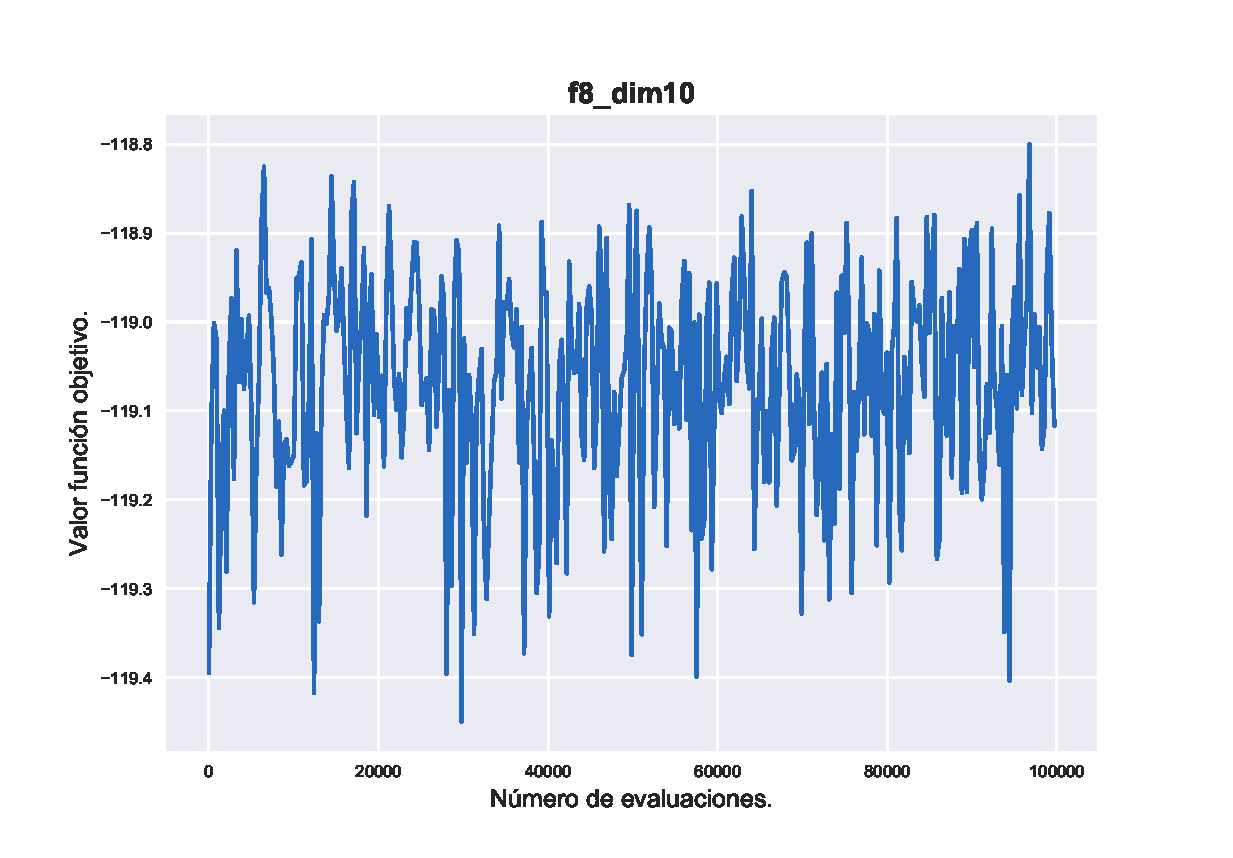
\includegraphics[width=0.5\linewidth]{./images/f8_dim10.eps} & 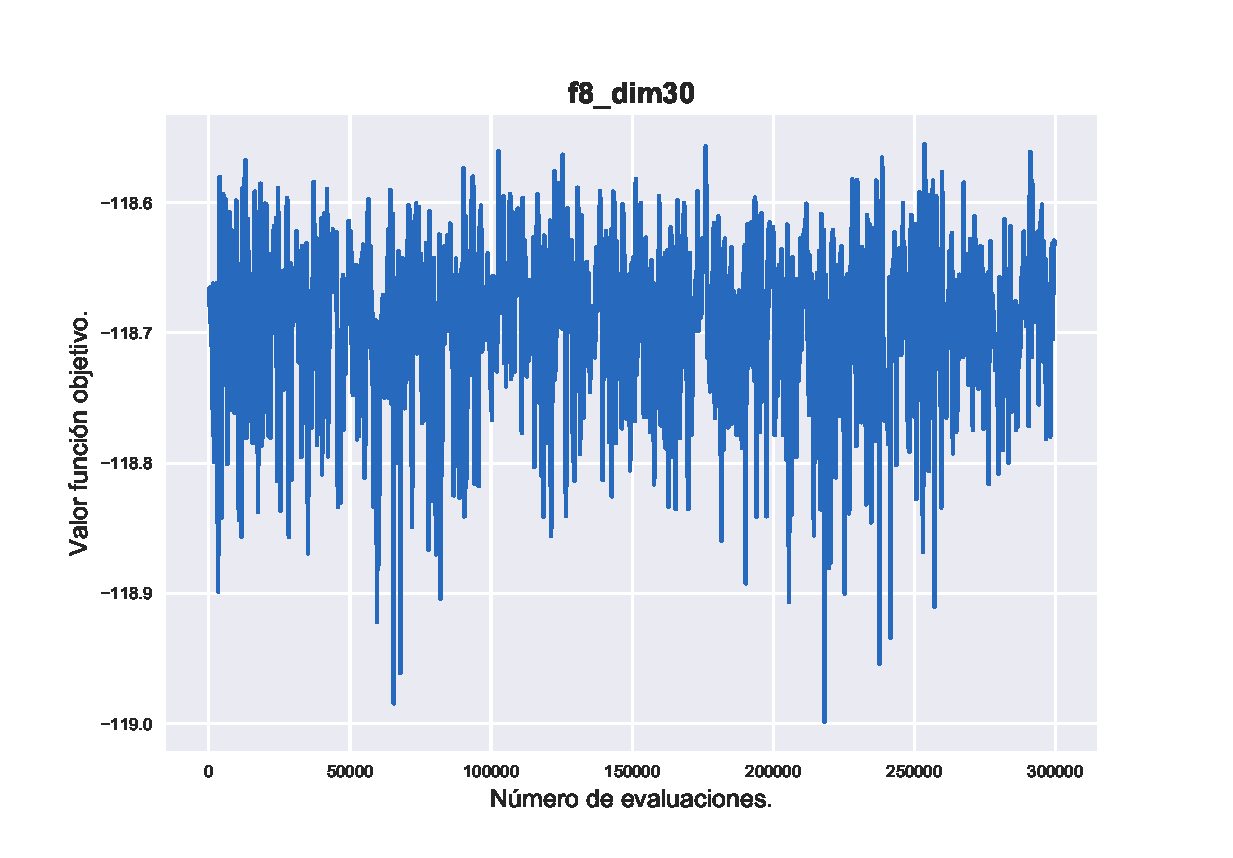
\includegraphics[width=0.5\linewidth]{./images/f8_dim30.eps} \\
	\end{tabular}
	\end{table}

	\begin{table}[H]
	\centering
	\begin{tabular}{ll}
	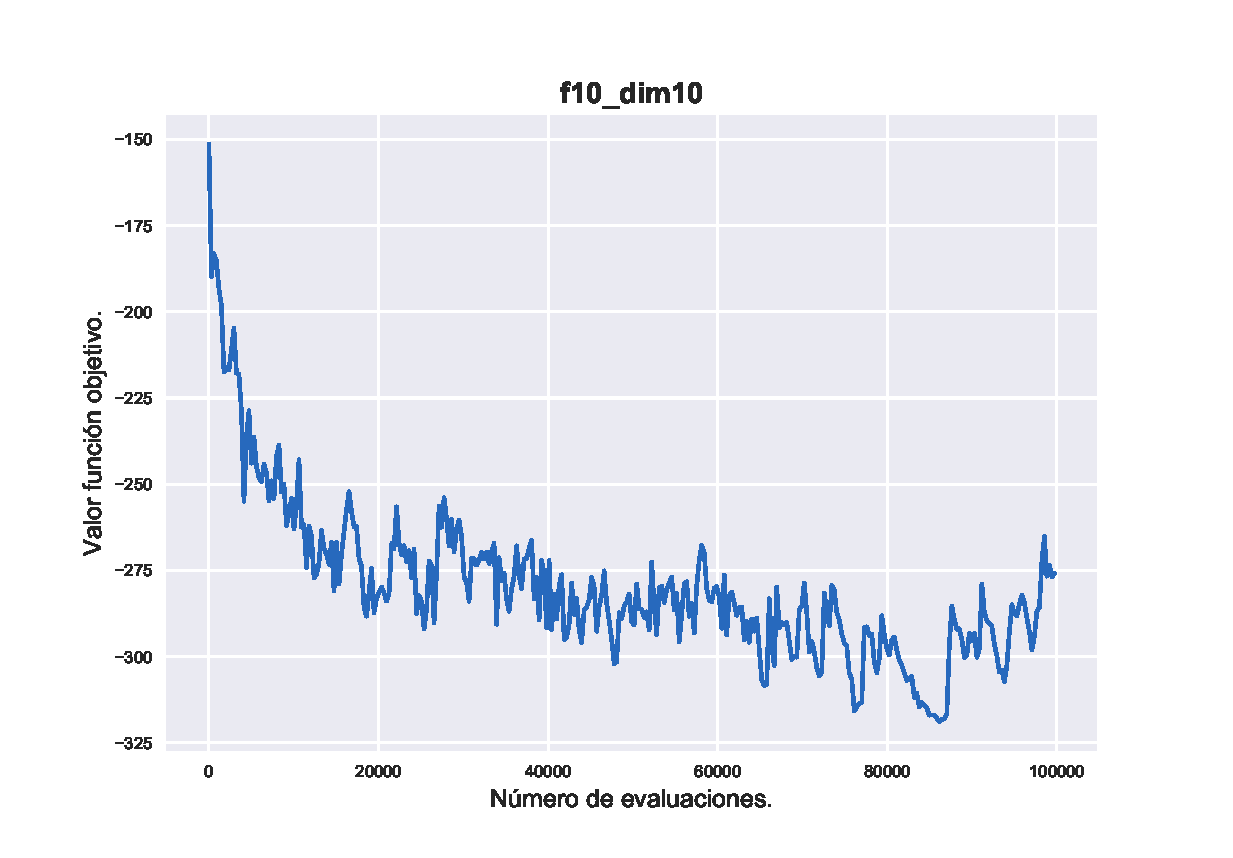
\includegraphics[width=0.5\linewidth]{./images/f10_dim10.eps} & 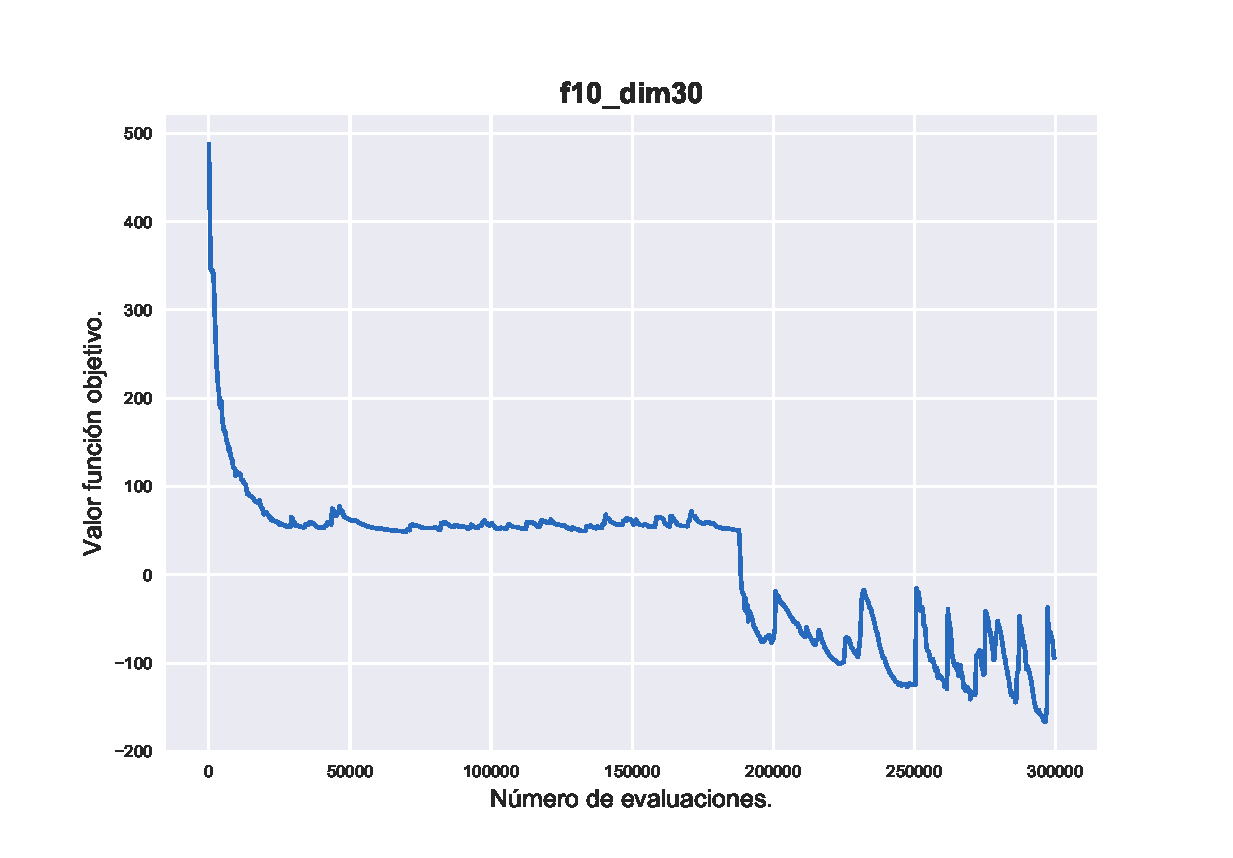
\includegraphics[width=0.5\linewidth]{./images/f10_dim30.eps} \\
	\end{tabular}
	\end{table}
	
	Hemos mostrado las gráficas de lo que sucede en tres casos distintos: en el caso de la función 5 que no se obtiene el mínimo podemos ver como el valor va descendiendo progresivamente acercándose al mínimo pero nunca llega a encontrarlo; en el caso de la función 8 podemos ver mucho movimiento del mejor valor por las zonas cercanas al óptimo, aunque no llega a encontrarlo, pero como podemos ver en la gráfica lo que sucede es que el algoritmo no es capaz de salir de esos mínimos locales; finalmente, en el caso de la función 10, para la cual casi obtiene el mínimo, podemos ver que el valor va descendiendo progresivamente y que hay momentos en los que se estanca pero luego es capaz de salir de esos mínimos locales. Para dimensión 30, aunque no se alcanza el óptimo, hay un punto interesante en la gráfica de convergencia. Cuando está llegando a las 200000 evaluaciones podemos ver que lleva un rato estancado y que, de repente, es capaz de salir del óptimo local y encontrar una solución bastante mejor. \\
	
	Queremos recalar que la mejor solución encontrada no es las última, si no el mínimo obtenido en todo el proceso de optimización. Es por ello que, siempre que se genera un nuevo mínimo mejor que el que llevamos hasta el momento, lo almacenamos y, una vez terminado el proceso de optimización, devolvemos ese mínimo almacenado.
	
	\section[Mejoras consideradas para el algoritmo genético.]{Mejoras consideradas para el algoritmo genético.}
	
	Una de las mejoras inmediatas que podemos considerar para un algoritmo genético es el reinicio de la población cuando detectamos que esta converge. Sin embargo, tras aplicar varias técnicas, la conclusión es que no es posible establecer un patrón para identificar cuando se debe reiniciar la población. De esta forma, los resultados obtenidos son, en general, peores que los obtenidos con el algoritmo básico. Las técnicas para detección de momentos de reinicio probadas son las siguientes:
	
	\subsection[Reinicio por diferencia de tamaño de partidos.]{Reinicio por diferencia de tamaño de partidos.}
	
	La idea es reiniciar la población cuando se detecta que el tamaño del partido con más individuos es un tanto por ciento mayor que el tamaño del partido con menos individuos. Es decir, consideramos que la población converge cuando la mayoría de individuos se encuentran en un partido, lo cual supone que dichos individuos sean similares. \\
	
	Los resultados obtenidos con esta técnica son, en el mejor de los casos iguales a los obtenidos sin ella. Podemos obtener una representación visual de lo que le sucede a la población durante el proceso de búsqueda representando los tamaños de los partidos mayoritarios y minoritarios frente al número de evaluaciones:
	
	\begin{table}[H]
	\centering
	\begin{tabular}{ll}
	\includegraphics[width=0.5\linewidth]{./images/restart_percentage_f1_dim10.eps} & \includegraphics[width=0.5\linewidth]{./images/restart_percentage_f5_dim10.eps} \\
	\end{tabular}
	\end{table}
	
	Como podemos ver, en el caso de la función 5 nunca se produce ningún reinicio  mientras que para la función 1 se produce un reinicio cuando la población lleva unas 180000 evaluaciones. El reinicio se puede ver en el pico donde ambas líneas de la función se vuelven a juntar.
	
	\subsection[Reinicio por estabilización del mejor individuo.]{Reinicio por estabilización del mejor individuo.}
	
	Esta técnica consiste en reiniciar la población cuando se detecta que el mejor individuo se estanca, es decir, no mejora con el paso de las iteraciones, lo que se traduce en que el proceso ha pasado de ser de exploración a ser de explotación. Representaremos gráficamente lo mismo que en la técnica anterior:
	
	\begin{table}[H]
	\centering
	\begin{tabular}{ll}
	\includegraphics[width=0.5\linewidth]{./images/restart_convergence_f1_dim10.eps} & \includegraphics[width=0.5\linewidth]{./images/restart_convergence_f8_dim10.eps} \\
	\end{tabular}
	\end{table}
	
	De nuevo, encontramos dos casos generales opuestos: un caso en el que nunca se produce un reinicio como sucede en la función 5 y otro en el que se produce un reinicio constante en las primeras etapas del algoritmo como sucede en la función 8, lo que en definitiva se traduce en buscar el mejor de entre una población de soluciones aleatorias de forma iterativa.
	
	\subsection[Reinicio por convergencia de la población.]{Reinicio por convergencia de la población.}
	
	Esta técnica consiste en reiniciar la población cuando se detecta que la diferencia entre el mejor individuo y el peor individuo es menor que un umbral, lo que se traduce en que todos los individuos de la población son muy similares y por lo tanto no hay diversidad que permita explorar nuevos entornos en el espacio de soluciones. Una vez mas los resultados obtenidos no mejora a los obtenidos con el algoritmo genético básico, por razones semejantes a las ya comentadas.
	
	\subsection[Conclusión.]{Conclusión.}
	
	A la vista de los resultados podemos concluir que, como era de esperar, determinar el umbral supone que una población se reinicie demasiadas veces, de forma que no converge y por tanto no encuentra un valor ni cercano al óptimo, o por el contrario no llega a reiniciarse y por tanto obtenemos los mismos resultados que con la versión básica del algoritmo genético. La elección del umbral que supone la reinicialización de la población es determinante para el comportamiento del algoritmo. Si establecemos un umbral demasiado bajo la población no se reiniciará y obtendremos los mismos resultados que con el algoritmo genético básico. Si establecemos un umbral demasiado alto podríamos tener más reinicios de los esperados lo cual supone un sobrecoste computacional y cambiar radicalmente el comportamiento del algoritmo de forma que este no es capaz de explorar apropiadamente un espacio de soluciones en el que encontrar la mejor.
\end{document}